\documentclass[10pt,letterpaper,twocolumn]{article}

\usepackage[margin=0.75in,columnsep=0.25in]{geometry}
\usepackage[T1]{fontenc}
\usepackage[utf8]{inputenc}
\usepackage{lmodern}
\usepackage{microtype}
\usepackage{amsmath,amssymb}
\usepackage{graphicx}
\usepackage{booktabs}
\usepackage{tabularx}
\usepackage{array}
\usepackage{enumitem}
\usepackage{xcolor}
\usepackage[round]{natbib}
\usepackage{xurl}
\usepackage[colorlinks=true,linkcolor=blue!60!black,citecolor=blue!60!black,urlcolor=blue!60!black]{hyperref}

\newcolumntype{L}{>{\raggedright\arraybackslash}X}
\setlist{itemsep=2pt,topsep=4pt}
\renewcommand{\refname}{Bibliography}
\setcounter{dbltopnumber}{2}
\renewcommand{\dbltopfraction}{0.85}
\renewcommand{\topfraction}{0.85}
\renewcommand{\textfraction}{0.1}
\renewcommand{\floatpagefraction}{0.8}
\renewcommand{\dblfloatpagefraction}{0.8}
\setlength{\emergencystretch}{1em}
\raggedbottom
\renewcommand{\bibfont}{\small\raggedright}
\setlength{\bibsep}{4pt plus 1pt}

\title{Countdown Clock Challenge: Learning NYC Subway Arrival Times}
\author{Yared Tsegaye Gizaw \and Alefew Yimam}
\date{Group 8\\[4pt]October 19, 2026}

\begin{document}
\maketitle

%======================================================================
\section{Motivation and Objectives}

\subsection{Problem definition and motivation}

New York riders plan around the subway countdown clock, but on the evening we measured it, its predictions 20--30 minutes ahead were off by 148~s on average, and trains came later than promised. We will build a deep learning model that predicts when each train will reach each of its next stops, up to 30 minutes ahead, and test it against the MTA's own live predictions on the same trains.

The MTA's clock drifts for a structural reason. Public descriptions of the lettered-line system say it relies on Bluetooth beacons at platform entrances and exits \citep{sas2016}. It ``only knows when a train has left or entered a station,'' so the countdown is ``an educated guess based on the scheduled time to get from one stop to the next'' \citep{gordon2018}.

When trains run slower than the schedule, because of slow zones, weekend track work or crowded platforms, a schedule-based estimate is optimistic, and the error grows with every stop further out. A model that learns how long trains actually take, and reacts to live conditions such as an overdue train or a slow train ahead, should drift less.

\paragraph{Task.} At a moment $p$, the input is everything the MTA feed has confirmed by $p$: the train's last confirmed stop and how long ago it was there, its recent stop-to-stop times, and where the other trains on the line are and how they have been running. The output is the arrival time at each later stop up to 30 minutes ahead. A train has \emph{arrived} at a stop when its first position report says it is stopped there; error is predicted minus actual arrival, in seconds.

\subsection{Objectives and what counts as success}

The project succeeds if our LSTM beats the MTA's countdown by at least 20\% for predictions 10--30 minutes ahead, on a held-out week, with a 95\% confidence interval that excludes zero.

\begin{enumerate}
  \item \textbf{Collect:} the MTA's predictions and train position reports from all 8 feeds every 30~s, Oct 20 -- Nov 15.
  \item \textbf{Baselines:} the MTA countdown, a history average and a gradient-boosted tree model.
  \item \textbf{Deep models:} a per-train LSTM (M1) and a line-wide model that sees every train on the line (M2).
  \item \textbf{Evaluate} every model on identical rows from a held-out week, by how far ahead it predicts.
  \item \textbf{Apply:} a live countdown board for one station showing the MTA's time and our side by side.
\end{enumerate}

\begin{table}[t]
  \centering
  \footnotesize
  \caption{Objectives and what counts as success.}
  \label{tab:success}
  \begin{tabularx}{\linewidth}{@{}>{\raggedright\arraybackslash}p{0.17\linewidth} L >{\raggedright\arraybackslash}p{0.27\linewidth}@{}}
    \toprule
    \textbf{Level} & \textbf{Criterion on the held-out week} & \textbf{Pilot evidence (Oct 18)} \\
    \midrule
    Must        & M1 cuts the MTA's error by $\geq$ 20\% at 10--30 min ahead (CI excludes 0) & 38--41\% lower \\
    Must        & M1 at most 5~s worse than the MTA at 0--2 min ahead & 25~s vs 35~s \\
    Should      & M1 beats the history average at every horizon (CI excludes 0) & Lower at all 5 horizons \\
    Stretch     & M2 beats the tree model at 10--30 min ahead (CI excludes 0) & Deep models tied the tree within 3~s \\
    Deliverable & Live board runs a full service day at one station & Logger and scorer work \\
    \bottomrule
  \end{tabularx}
\end{table}

%======================================================================
\section{Related Work}

% page-wide floats for Section 3 (placed here so they land next to it)
\begin{table*}[t]
  \centering
  \small
  \caption{Models and novelty.}
  \label{tab:models}
  \begin{tabularx}{\textwidth}{@{}>{\raggedright\arraybackslash}p{0.14\textwidth} L >{\raggedright\arraybackslash}p{0.27\textwidth} >{\raggedright\arraybackslash}p{0.17\textwidth}@{}}
    \toprule
    \textbf{Model} & \textbf{What it does} & \textbf{Inputs} & \textbf{Course concepts used} \\
    \midrule
    B0 MTA countdown & The feed's own prediction & The MTA's own & --- \\
    \addlinespace
    B1 History average & Last confirmed stop + median stop-pair travel time by line, direction, time of day and day type & Stop pair, clock time & --- \\
    \addlinespace
    B2 Gradient-boosted trees & Corrects B1 using 23 features: 15 hand-made plus the last 8 stop-to-stop delays & Time since last stop, how overdue, recent delays, gap to and delay of the train ahead & --- \\
    \addlinespace
    M1 Per-train LSTM & LSTM (32 units) over the last 8 stop-to-stop delays, joined with B2's features and a line embedding, then a 2-layer MLP & Same as B2, delays as a sequence & LSTM, Adam, dropout, batch norm, Xavier init \\
    \addlinespace
    M2 Line-wide model & Bidirectional LSTM over every train on the line at moment $p$, ordered along the route; predicts all later stops in one pass & The above for all trains on the line and shared-track lines; alerts (optional) & LSTM; transformer encoder as an extension \\
    \bottomrule
  \end{tabularx}
\end{table*}

\begin{figure*}[t]
  \centering
  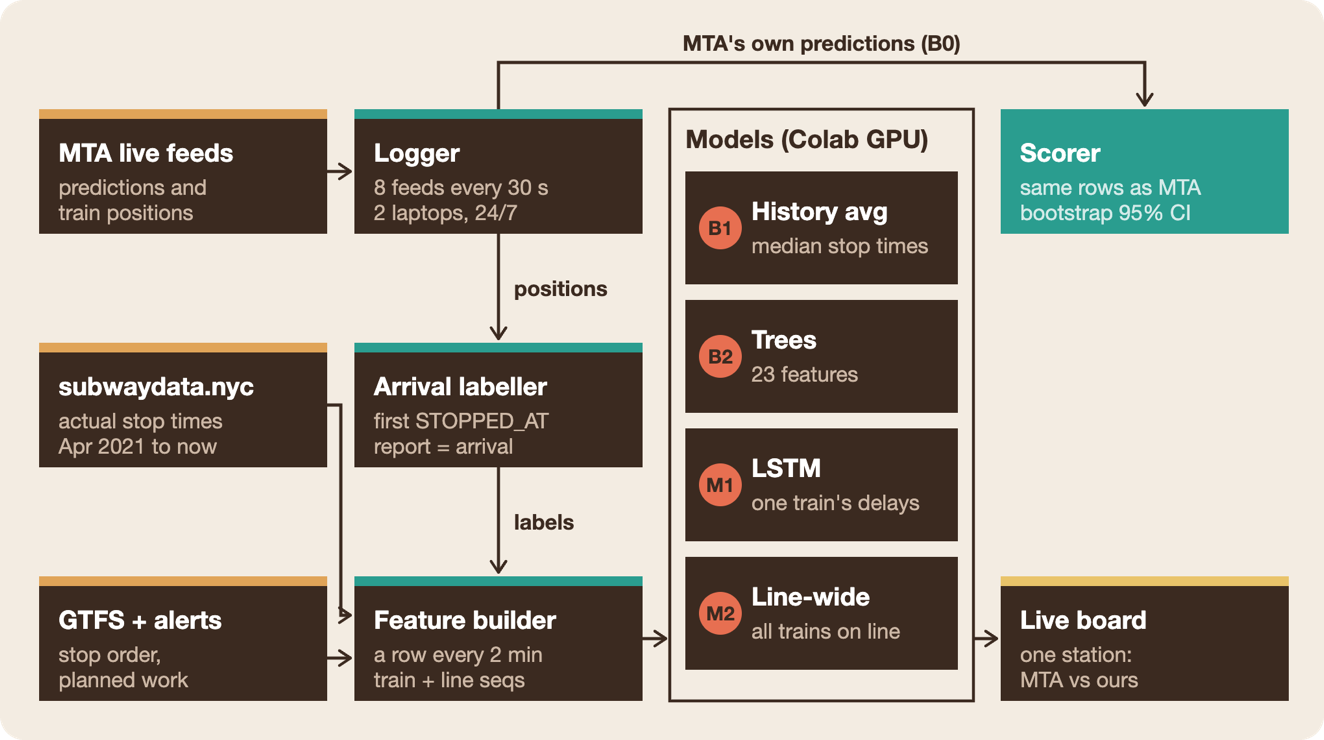
\includegraphics[width=0.66\textwidth]{figures/fig1-system-design.png}
  \caption{\textbf{Every model, the MTA included, is scored on rows from one recording.} System architecture: components and how data flows between them.}
  \label{fig:system}
\end{figure*}


We found no published study of how accurate NYC subway countdowns are at different horizons. In 2017 the MTA called its lettered-line system ``97 percent accurate'' but gave no method \citep{ny1_2017}. Public descriptions say it combines platform beacons with scheduled stop-to-stop times \citep{sas2016,gordon2018}. We measure its error against its live predictions, horizon by horizon.

\citet{newmark2024} measured how accurate GTFS-Realtime arrival predictions were at California transit agencies; we study the NYC subway and add a model that improves on the agency's predictions. \citet{rashvand2023} predicted NYC bus arrivals with a fully connected network, under 40~s error across 200+ lines; we use sequence models for the subway. \citet*{luo2023} predicted delays of several high-speed-rail trains at once with an FCNN plus two LSTMs (MAE 1.379 min); our line-wide model applies that many-trains idea to a dense urban subway. History comes from \href{https://subwaydata.nyc/}{subwaydata.nyc}, an archive of actual stop times since Apr 1, 2021, which we relabel with position reports (Section~\ref{sec:data}).

Our models build on the LSTM \citep{hochreiter1997} and, as an extension beyond the course list, the transformer \citep{vaswani2017}. The strongest non-deep baseline is gradient boosting \citep{friedman2001}.

%======================================================================
\section{Proposed Work}

\subsection{Data and ground truth}
\label{sec:data}

All our data is public and free. The one thing nobody archives is the MTA's own past predictions, so we record those ourselves.

\begin{itemize}
  \item \textbf{MTA GTFS-Realtime feeds (all 8):} the MTA's predicted arrivals and train position reports. We record them every 30~s, Oct 20 -- Nov 15 ($\approx$225 MB/day compressed); public endpoint, no API key.
  \item \textbf{\href{https://subwaydata.nyc/}{subwaydata.nyc}:} actual stop times for every trip since Apr 1, 2021 ($\approx$1.4 MB/day), as daily CSV downloads.
  \item \textbf{MTA static GTFS and service alerts (data.ny.gov):} stop order for each line, and planned-work notices since Apr 2020 as an optional input for M2.
\end{itemize}

\paragraph{Ground truth.} A train \emph{arrives} at a stop at its first position report with status \texttt{STOPPED\_AT}, ``the vehicle is standing at the stop'' in the \href{https://gtfs.org/documentation/realtime/reference/}{GTFS Realtime reference}. History archives like subwaydata.nyc instead record the last time the feed listed for a stop before dropping it. In our pilot that ran 30~s late on numbered lines and 75~s late (median) on lettered lines, roughly one platform stop, and made the MTA look worse at short range than it is. We therefore score against position reports, pretrain on 2021--2026 history under its own definition, and learn a per-station correction fitted only on our logged training weeks.

\paragraph{Prediction rows.} Every 2 minutes, for every train in service, we make one row per later stop it will reach within 30 minutes. Every model, the MTA included, is scored on exactly these rows; the pilot produced about 1,000 rows per minute of Sunday-evening service.

\subsection{Models and novelty}

Each model has to beat the one above it; all learned models predict actual minus typical travel time with absolute-error (L1) loss. The real test for the deep models is the tree baseline, which tied our per-train LSTM in the pilot.

\paragraph{What is new.}
\begin{itemize}
  \item \textbf{A fair head-to-head with the MTA:} same trains, same moments, arrival from position reports. No per-horizon comparison like this has been published for the NYC subway.
  \item \textbf{Line-wide state:} in the pilot, three very different per-train models finished within 3~s of each other, so the inputs were the limit. M2 tests whether seeing a delay build several trains ahead lets a deep model beat the tree.
  \item \textbf{Five years of public history, made consistent} with the position-report definition of arrival, using weeks we record ourselves.
\end{itemize}

\subsection{System design}

% pilot chart first, so figures stay numbered in reading order
\begin{figure}[t]
  \centering
  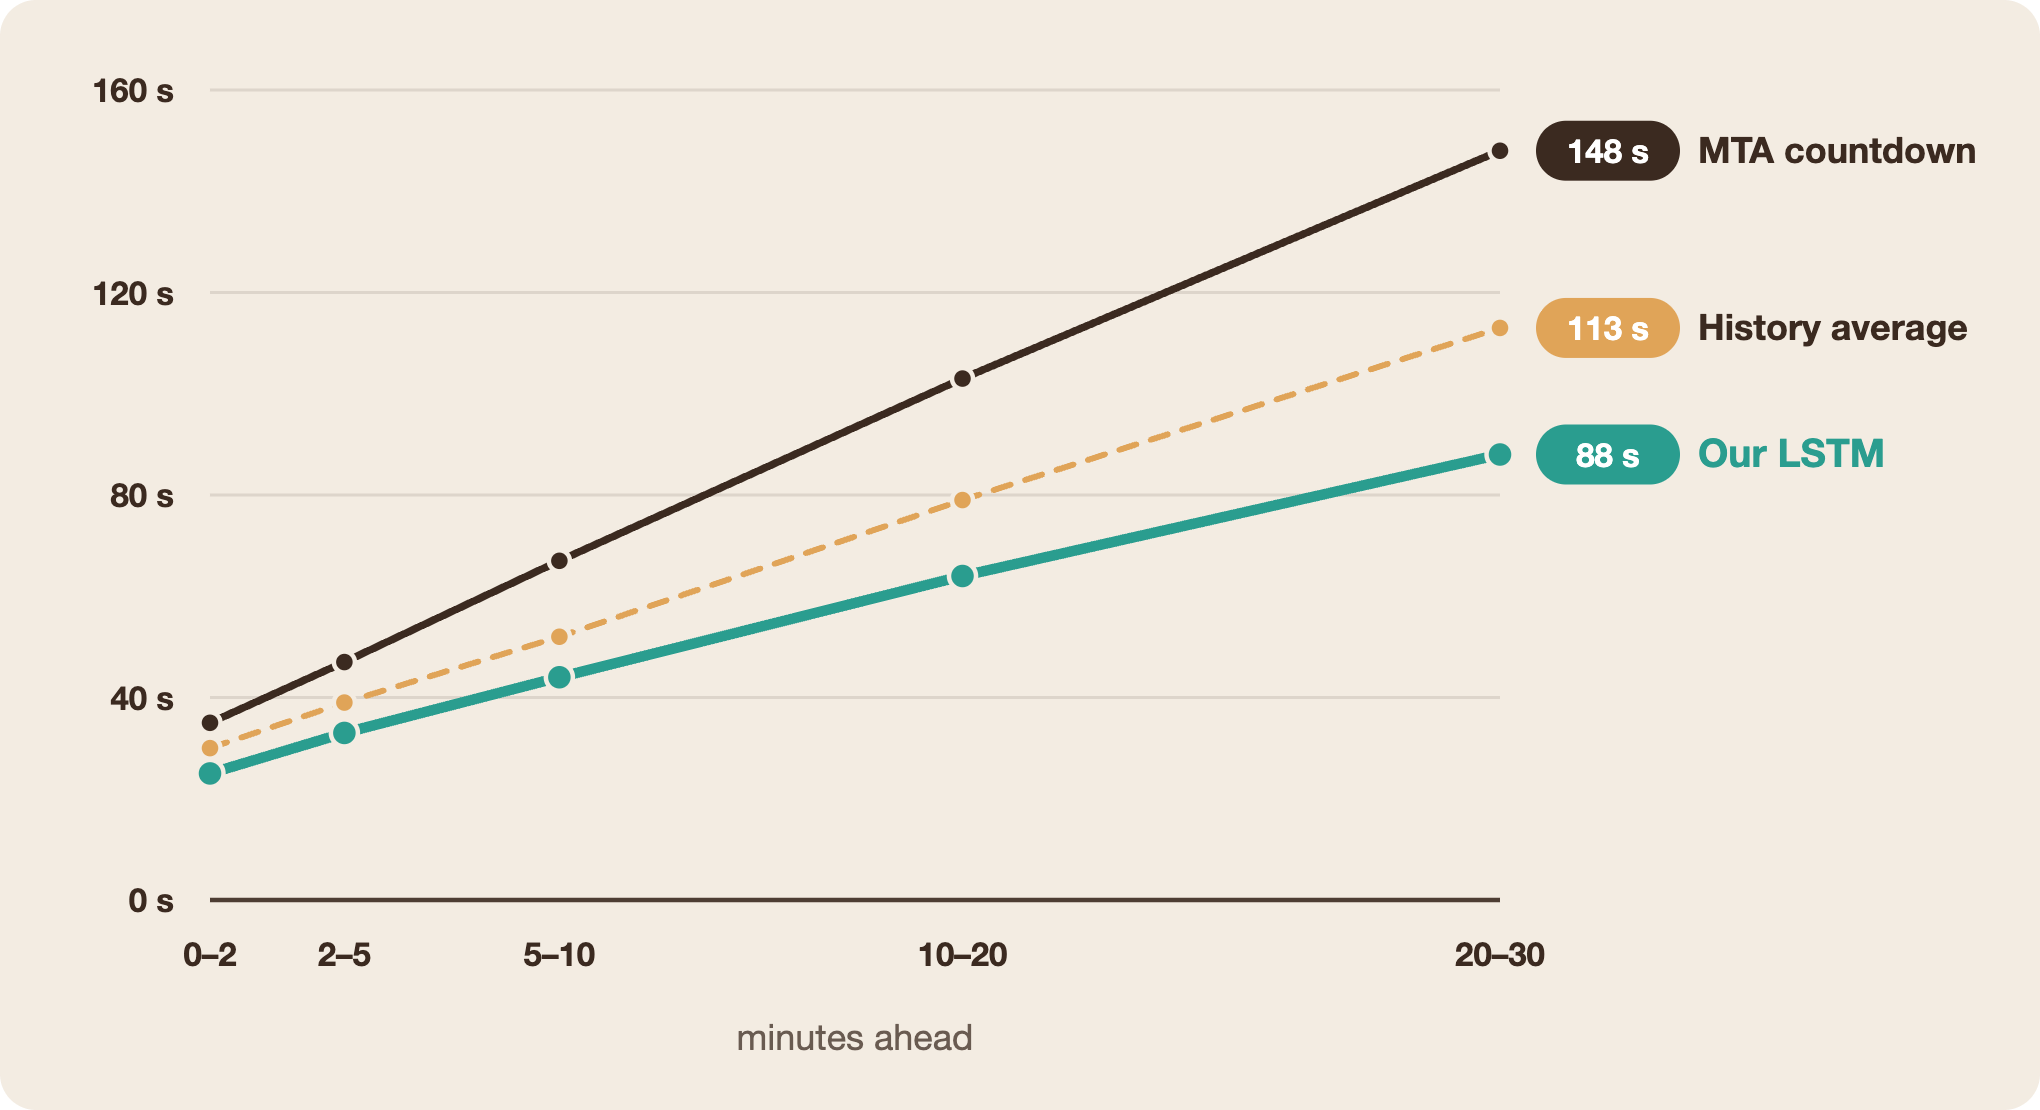
\includegraphics[width=\linewidth]{figures/fig2-pilot-results.png}
  \caption{\textbf{Our LSTM's error grows far more slowly than the MTA'S countdowns.} Mean absolute error in seconds, by how far ahead the prediction was made $\cdot$ 49,380 predictions. Pilot recording, Sun Oct 18 2026, 7:37--8:57 PM, 424 trains on all lines; arrival from position reports.}
  \label{fig:pilot}
\end{figure}

% page-wide floats for Section 4 (placed here so they land next to it)
\begin{figure*}[t]
  \centering
  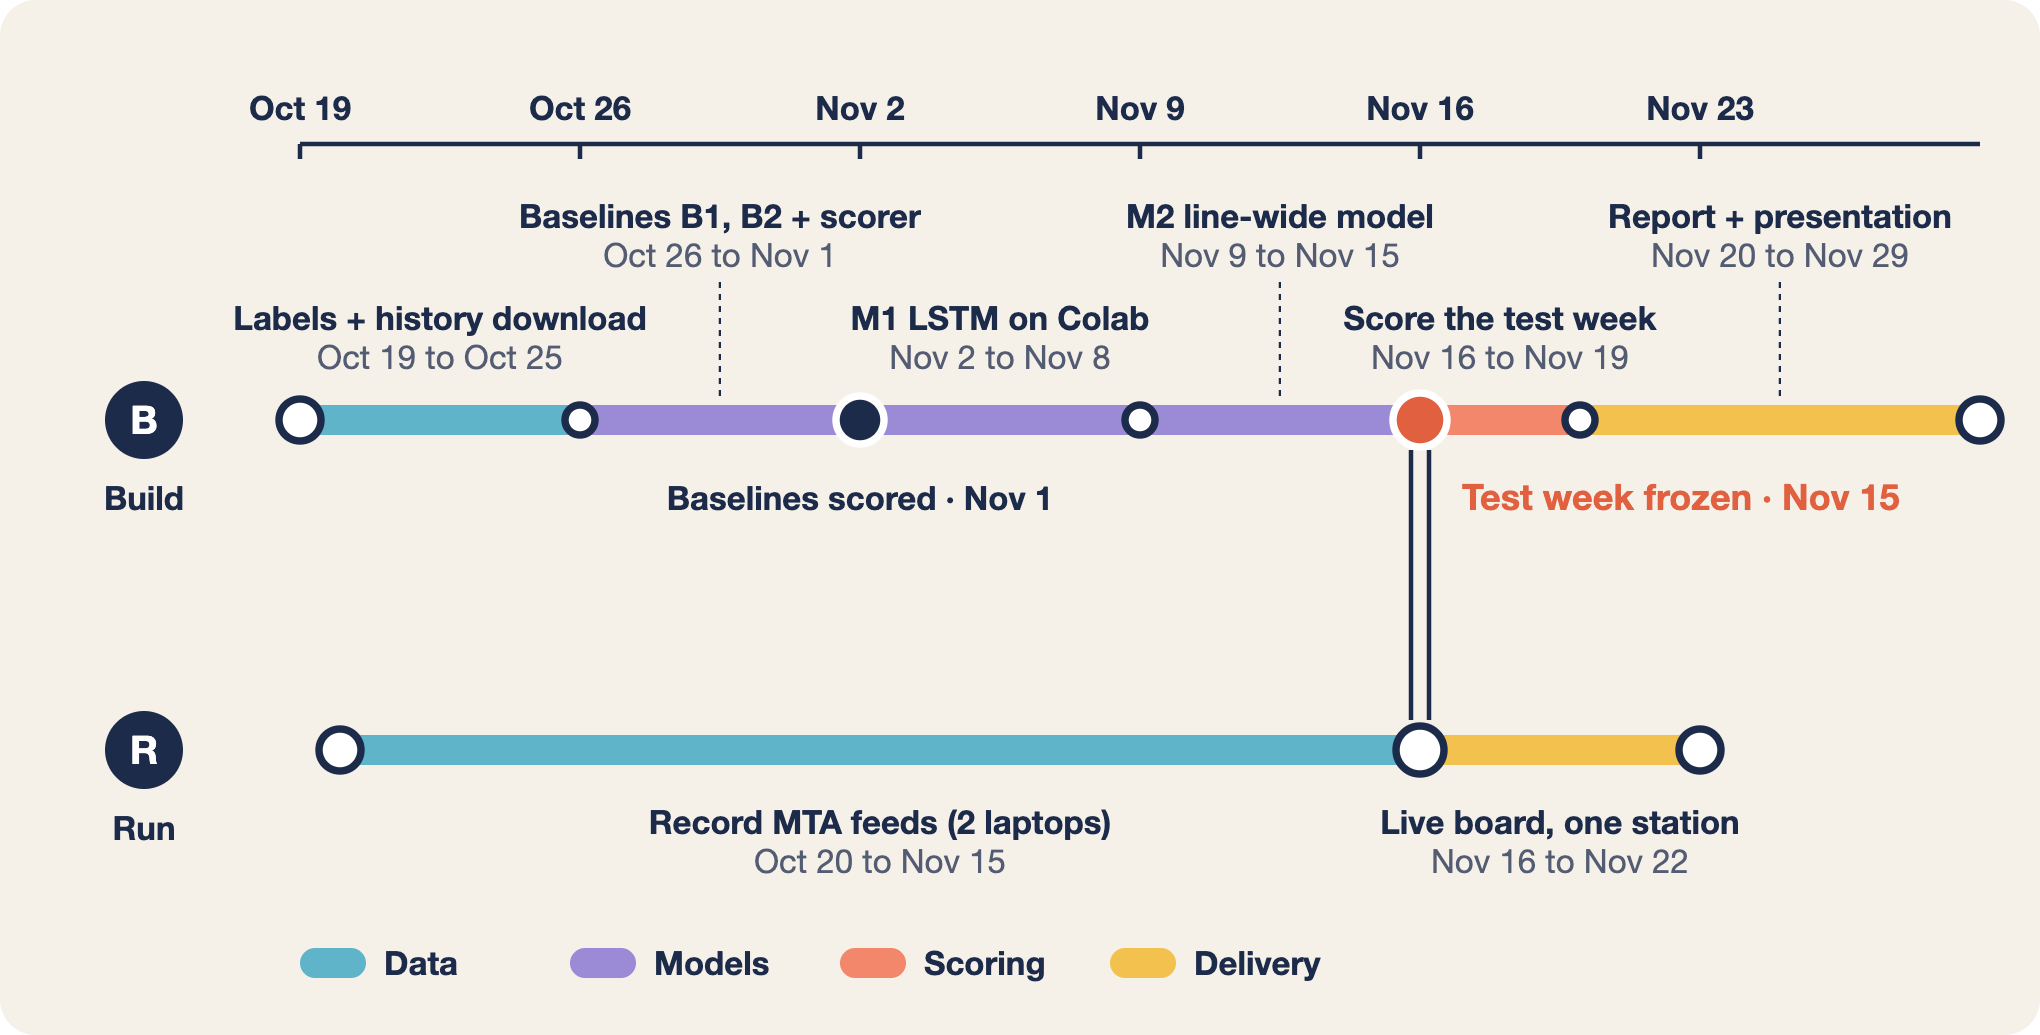
\includegraphics[width=0.72\textwidth]{figures/fig3-schedule.png}
  \caption{\textbf{The test week is recorded and frozen by Nov 15, leaving two weeks to score and write up.} Weekly plan, 2026 $\cdot$ two parallel tracks meet when the test week is frozen. Project schedule, Oct 19 -- Nov 29, 2026.}
  \label{fig:schedule}
\end{figure*}

\begin{table*}[t]
  \centering
  \small
  \caption{Division of work.}
  \label{tab:division}
  \begin{tabularx}{\textwidth}{@{}L l l L@{}}
    \toprule
    \textbf{Workstream} & \textbf{Lead} & \textbf{Support} & \textbf{Deliverable} \\
    \midrule
    Recording and storage & Yared Tsegaye & Alefew Yimam (second logger) & 4 weeks of recordings on Drive \\
    Arrival labels, history correction & Yared Tsegaye & --- & Labelled train, validation, test sets \\
    Baselines B1, B2 and the scorer & Yared Tsegaye & Alefew Yimam reviews & Scorer with bootstrap intervals \\
    LSTM M1 and line-wide model M2 & Alefew Yimam & Yared Tsegaye reviews & Trained models on Colab \\
    Live countdown board & Alefew Yimam & Yared Tsegaye & Board running at one station \\
    Report and presentation & Both & --- & Each writes their own sections \\
    \bottomrule
  \end{tabularx}
\end{table*}


The logger takes two things from the same feed. The MTA's predictions go straight to the scorer as baseline B0, and the position reports become our arrival labels. At run time, the same feature builder turns the live feed into rows for the board.

\subsection{Pilot results (Oct 18)}

A working prototype already beats the MTA. On Sunday, Oct 18 we recorded the MTA's predictions for 80 minutes and trained our models on 2.8 million examples from Aug 8 -- Oct 17 history. We then scored every model on the MTA's own rows.

The tree model and a transformer finished within 3~s of the LSTM at every horizon, which is why M2 adds line-wide state. Two caveats bound the result: it is a single Sunday evening with planned work, likely the MTA's worst case, and the models were shifted 30~s (numbered lines) and 75~s (lettered lines) onto the position-report definition using offsets measured that same night.

%======================================================================
\section{Plan of Action}

\subsection{Resources}

Everything we need is free or already in hand. Data comes from the public MTA feeds (no API key) and the subwaydata.nyc archive. Two of our own laptops record 24/7, because Colab sessions time out, and about 6 GB of recordings go on our university Google Drive. We train on Colab GPUs (free/Pro, already available) with Python, PyTorch, pandas, scikit-learn and gtfs-realtime-bindings, starting from the logger, scorer and training scripts written for the Oct 18 pilot. The one hard requirement is a logger running non-stop from Oct 20.

\subsection{Weekly schedule and milestones}

No model sees the test week until Nov 16. M2 is built while that week is still being recorded.

\subsection{Division of work}

Yared Tsegaye owns the data and the scoring, and Alefew Yimam owns the models and the board, so neither one grades their own model.

\subsection{Risks and mitigations}

The biggest risk is that our deep models only tie the tree baseline, as they did in the pilot.

\begin{itemize}
  \item \textbf{Deep models only tie the tree.} M2 adds information the tree lacks; if it still ties, we report that as a finding.
  \item \textbf{A logger stops (laptop sleeps, Wi-Fi drops).} Two laptops record in parallel and we merge them; gaps are excluded for every model alike.
  \item \textbf{The pilot evening flattered us.} The test week includes weekday rush and results are split by period; rerouted trains and noisy labels are covered by the checks in Section~\ref{sec:eval}.
\end{itemize}

%======================================================================
\section{Evaluation and Testing Method}
\label{sec:eval}

The final verdict comes from a single held-out week, Nov~\mbox{9--15}, that no model sees during training or tuning. We score it once, at the end. Models pretrain on subwaydata.nyc history (Apr 2021 -- Oct 19), train on our recordings from Oct 20 -- Nov 1 (which also fit the arrival-definition correction), and use Nov 2--8 for early stopping and model choice.

\paragraph{Metrics.} In five horizon bands (0--2, 2--5, 5--10, 10--20 and 20--30 min ahead) we report mean absolute error in seconds, the share of predictions within 60~s, and mean signed error, which shows whether a model is too optimistic. Each is split by numbered vs lettered lines and by weekday rush (7--10 am and 4--7 pm), other weekday hours, and weekends.

\paragraph{Statistics.} Every difference between two models gets a 95\% confidence interval from a bootstrap that resamples whole trains (500 resamples). Predictions for the same train are correlated, so resampling single rows would make the intervals too narrow \citep{efron1993}.

\paragraph{Checks.} We re-score under the ``last reported time'' definition of arrival, which should not flip the conclusions. We report what share of the MTA's rows each model could score, with rerouted trains shown separately. Veterans Day (Wed Nov 11) falls in the test week, so we report it separately as well as in the totals.

\paragraph{Live test.} The countdown board runs for one full service day at one station. Both clocks are logged and scored against the position-report arrivals.

%======================================================================
\nocite{*}
\bibliographystyle{plainnat}
\bibliography{references}

\end{document}
